%--------------------------------------------------------------------------------------------------
\chapter{Einleitung} \label{cha:Einleitung}	

\lipsum[1]

%--------------------------------------------------------------------------------------------------
\section{Motivation}\label{sec:Motivation}

\lipsum[1]

%--------------------------------------------------------------------------------------------------
\section{Zielsetzung}\label{sec:Zielsetzung}

\lipsum[1]
bla bla bla bla bla bla bla bla bla bla bla bla bla bla bla bla bla bla bla bla bla
bla bla bla bla bla bla bla bla bla bla bla bla bla bla bla bla bla bla bla bla bla
bla bla bla bla bla bla bla bla bla bla bla bla bla bla bla bla bla bla bla bla bla
bla bla bla bla bla bla bla bla bla bla bla bla bla bla bla bla bla bla bla bla bla

%--------------------------------------------------------------------------------------------------
\section{Aufbau der Arbeit}\label{sec:AufbauDerArbeit}
Der Aufbau dieser Arbeit ist in Abbildung \ref{fig:AufbauDerArbeit} dargestellt.
\begin{figure}[h]
	\centering
	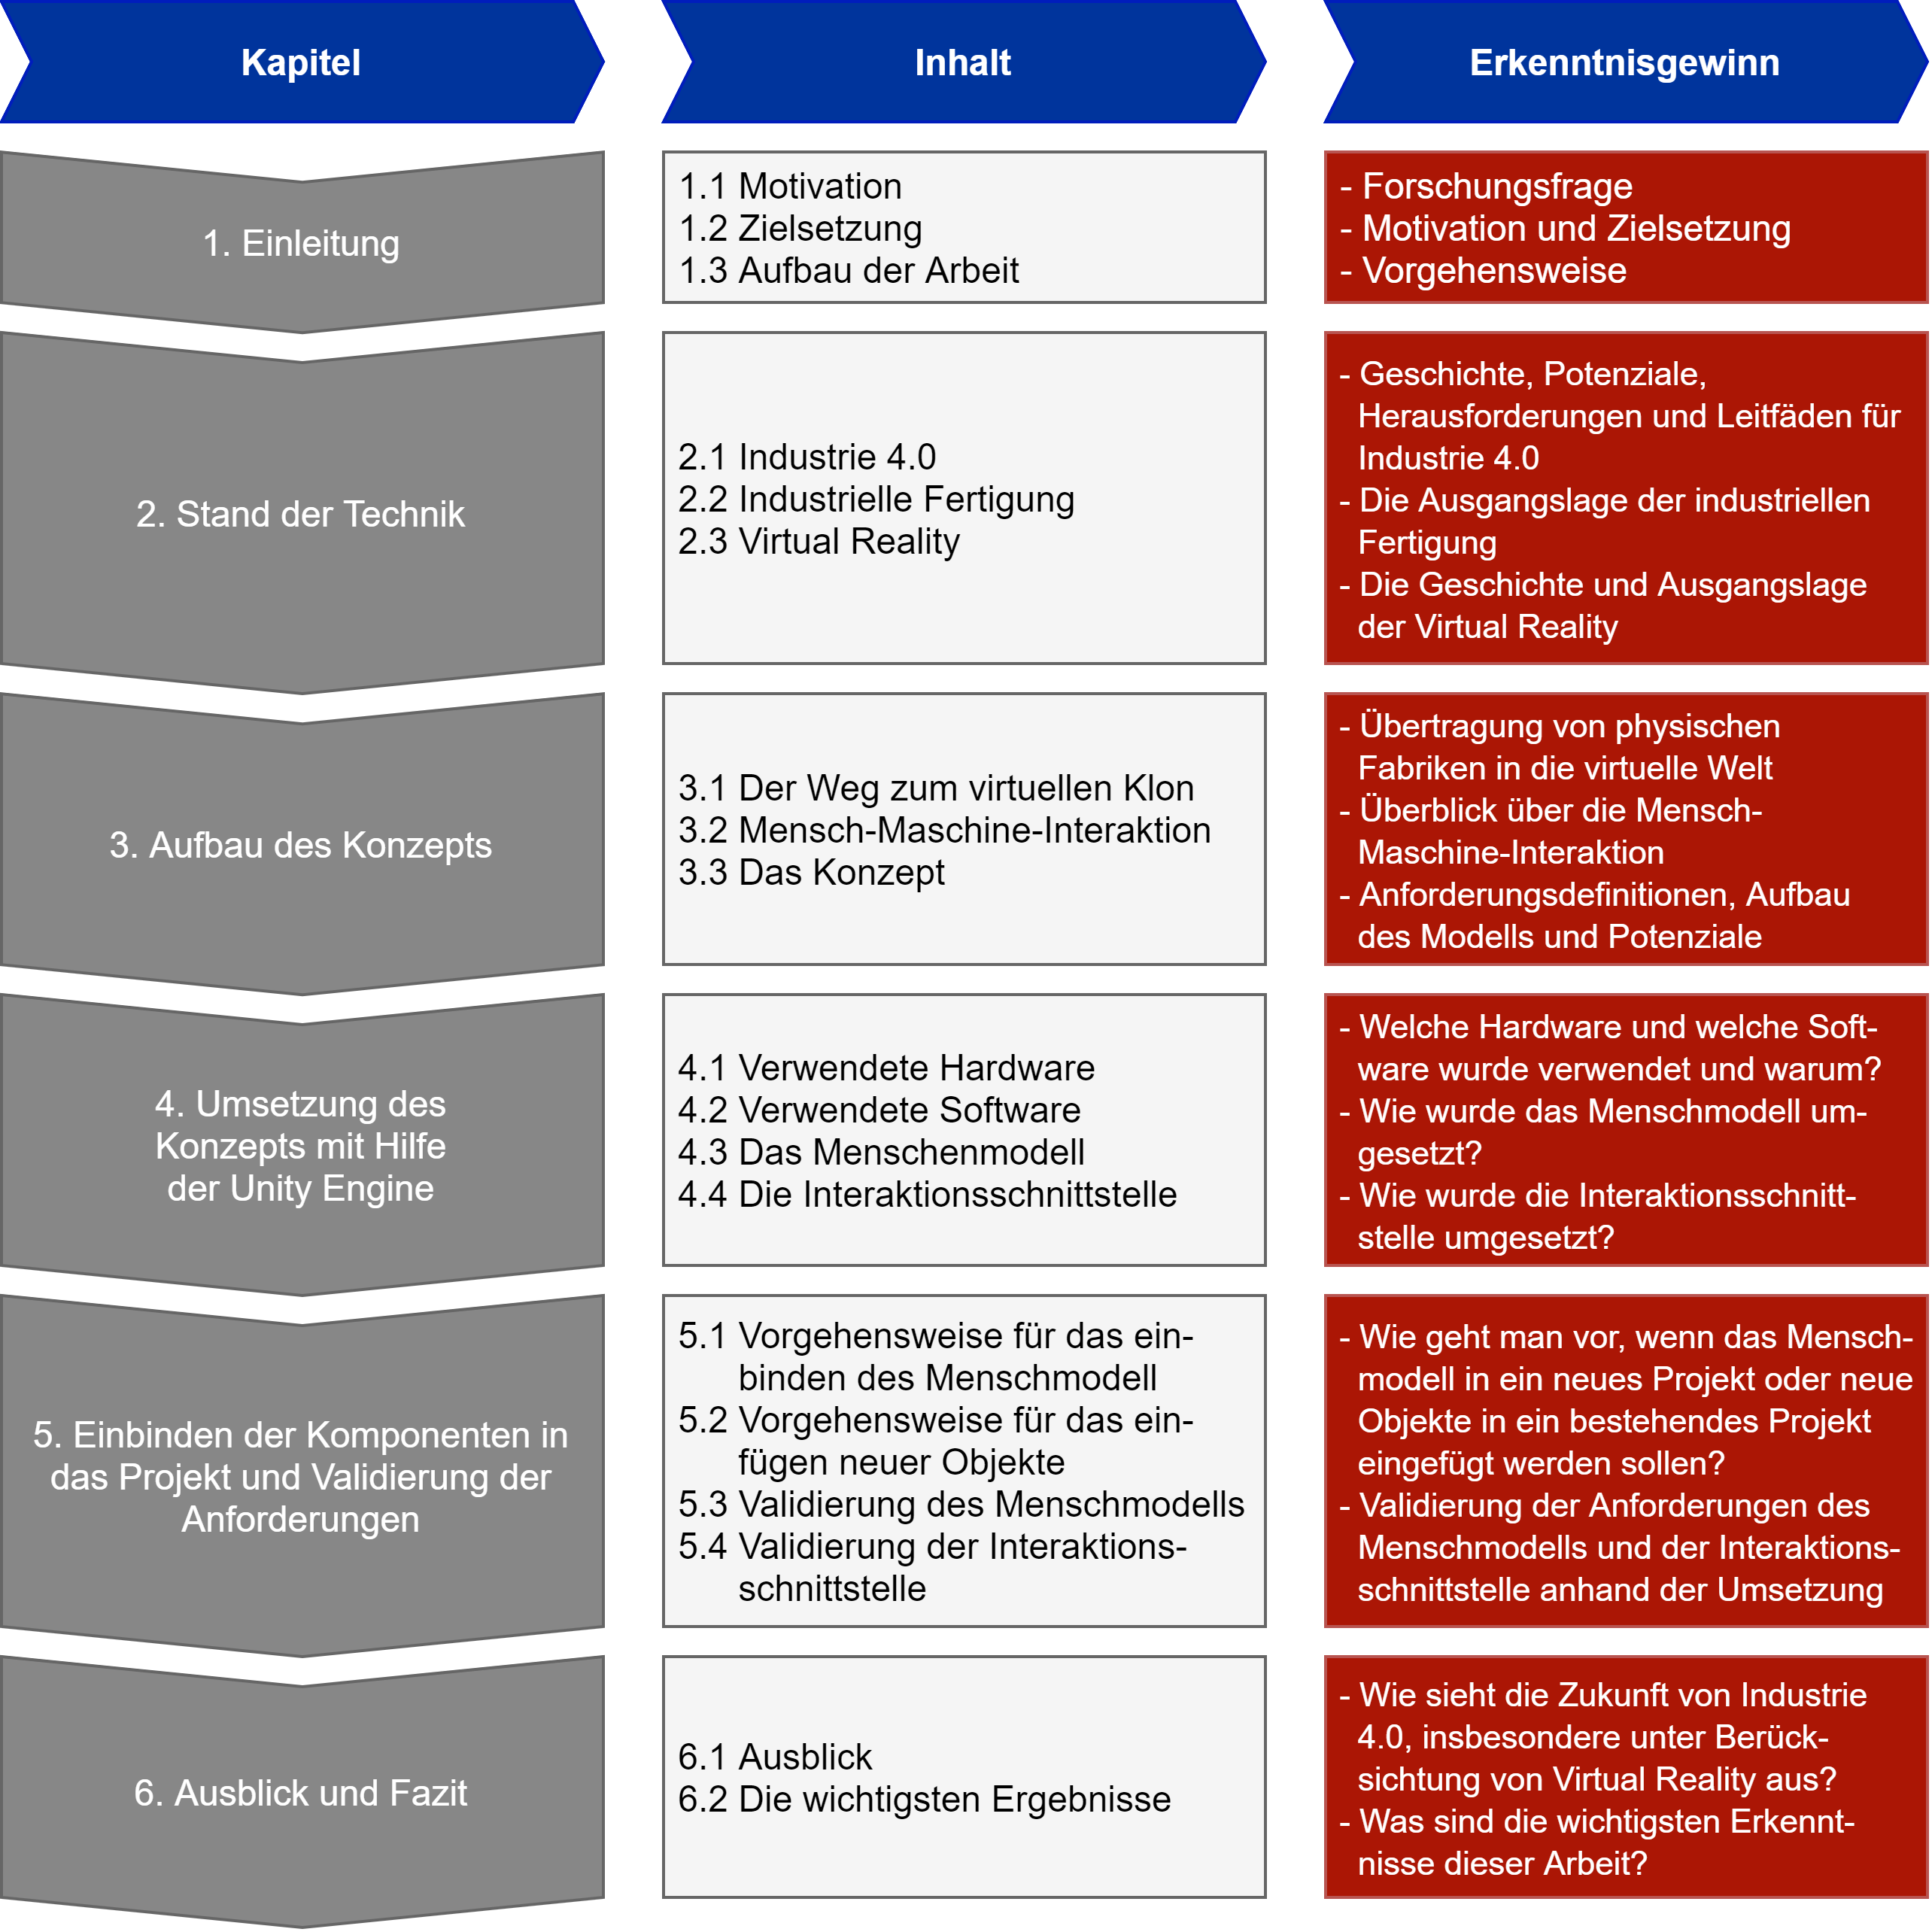
\includegraphics[width=1\linewidth]{Bilder/A55_AufbauNeu}
	\caption{Der Aufbau der Arbeit, eigene Abbildung}
	\label{fig:AufbauDerArbeit}
\end{figure}
\newline
Zunächst wird, nach der Einleitung, in Kapitel XX der aktuelle Stand der Technik thematisiert. Konkret gibt es zu Beginn des Kapitels einen Einblick in die Geschichte der industriellen Revolutionen und der Wandlungen im Bereich der Informations- und Kommunikationstechnik (Kapitel XX), bevor anschließend die Potenziale (Kapitel XX) und Herausforderungen (Kapitel XX) von Industrie 4.0 erläutert werden. Schließlich gibt es noch eine Einführung in zwei Leitfäden, die Unternehmen bei dem Wandel zu Industrie 4.0 unterstützten sollen (Kapitel XX).
\newline
Im darauf folgenden Kapitel XX wird das übergeordnete Konzept erläutert. Aufgrund dessen wird zunächst der Prozess von der physischen Produktionsanlage bis hin zu ihrem virtuellen Klon erläutert (Kapitel XX) und die Arbeit in diesem Prozess eingeordnet. Daraufhin gibt es einen Überblick über die Mensch-Maschine-Interaktion im Kontext dieser Arbeit (Kapitel XX), bevor auch in diesem Kapitel die Arbeit entsprechend eingeordnet wird. Anschließend wird das eigentliche Konzepts des Menschmodells aufgebaut (Kapitel XX), indem zunächst die Anforderungen an das Menschmodell und die Interaktionsschnittstelle erläutert werden (Kapitel XX). Des Weiteren gibt es eine Einführung in das Functional-Mockup Interface (Kapitel XX), bevor erläutert wird, wie die Umsetzung des Menschmodells mit Hilfe des FMI Standards auszusehen hätte (Kapitel XX) und worin die Potenziale liegen würden (Kapitel XX).
\newline
Aufbauend auf den in Kapitel XX gewonnen Verständnis und insbesondere unter Berücksichtigungen der in Kapitel XX gestellten Anforderung wird in Kapitel XX die eigentliche Umsetzung des Konzepts mit Hilfe der Unity Engine erläutert. Aufgrund dessen gibt es zunächst eine Einführung in die Verwendete Hardware (Kapitel XX) und Software (Kapitel XX), bevor Anschließend die eigentliche Umsetzung des Menschmodells (Kapitel XX) und der Interaktionsschnittstelle (Kapitel XX) erläutert werden.
\newline
In Kapitel XX gibt es zunächst eine Einführung in die Vorgehensweise beim Einbinden des Menschmodells und der Interaktionsschnittstelle in ein neues Projekt (Kapitel XX), bevor anschließend die Vorgehensweise beim Einfügen neuer Objekte in der Umgebung erläutert wird (Kapitel XX). Schließlich werden in Kapitel XX und XX die in Kapitel XX gestellten Anforderungen an das Menschmodell und die Interaktionsschnittstelle, unter Berücksichtigung der in Kapitel XX erläuterten Umsetzung des Konzepts, validiert.
\newline
Abschließend gibt es in Kapitel XX einen Ausblick (Kapitel XX), der sich damit befasst wie die Zukunft von Industrie 4.0, insbesondere im Hinblick auf Virtual Reality, aussehen könnte. Des Weiteren werden die wichtigsten Erkenntnisse der Arbeit zusammengefasst (Kapitel XX).

%--------------------------------------------------------------------------------------------------